\chapter{Experimentación y Resultados}
\label{chapter:experimentacion_resultados}

\section{Conjuntos de datos}

Para comenzar la experimentación vamos a hacer un repaso de los conjuntos de datos y la técnica seguida para realizar la misma. En primer lugar cabe decir que al ser un problema no supervisado en origen no tendríamos forma de saber nuestro acierto en el problema. En este tipo de casos hay dos aproximaciones: estimar el acierto o utilizar conjuntos que sí están clasificados y obtener de esta forma el acierto. La segunda de las alternativas es la que vamos a seguir en este estudio y es la que se suele denominar como problema semisupervisado. 

Para tomar este camino necesitamos conjuntos en los que tengamos disponible la clasificación de datos anómalos y no anómalos. Estos conjuntos de datos han sido tomados de la web Otlier Dection Datasets \cite{shebuti_ryana_odds_2016}, librería mantenida por la universidad Stony Brooks.

Estos conjuntos de datos están en formato Matlab, formato que puede ser fácilmente leído por la librería SciPy. Estos conjuntos de datos vienen con información de cabecera, versión e incluso algunos con una breve descripción o resumen si dispusieran de ella. Lo importante es que los datos vienen divididos en dos, primero un vector que contiene una lista con los vectores que componen los datos y en segundo lugar un vector con las etiquetas donde $0$ significa que el dato no es anómalo y $1$ que sí lo es.

\begin{figure}[H]
	\centering
	\label{dataset_matlab}
	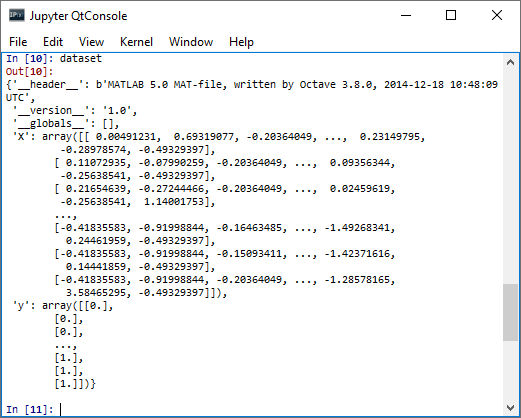
\includegraphics[scale=0.8]{imagenes/datasets_matlab}
	\caption{Contenido de los conjuntos de datos}
\end{figure}

Como podemos ver ``X'' contiene el conjunto de datos y el campo ``y'' contiene las etiquetas para los mismos.

En algunos de estos conjuntos de datos podemos encontrar lo que conocemos como valores perdidos o en inglés ``missing values''. Estos valores vienen reflejados con ``NAN'' en los conjuntos. Estos valores no sólo no nos son de interés si no que además nuestros modelos no están preparados para poder trabajar con ellos por lo que tenemos que decidir que transformación aplicamos para poder emplear los conjuntos de datos. La decisión tomada para estos valores ha sido la de eliminar las instancias que presenten valores perdidos. Esta decisión se basa en que, si estas instancias son anómalas no tenemos forma alguna de tratar con ellas porque no disponen de valores numéricos en sus campos y por tanto nuestros modelos no son aptos para resolver el conflicto. Esto no excluye el hecho de que estas instancias puedan ser anomalías reales. Por ejemplo pensemos en un sistema de frenos que sufre una rotura de alguno de sus sistemas. Si estos sistemas poseen sensores que recopilan datos es muy probable que estos sensores no tomen valores y por tanto dispongamos de valores perdidos precisamente porque la instancia es anómala. Esto se discutirá un poco más en profundidad cuando hablemos del trabajo futuro, de momento la decisión ha sido suprimir estas instancias.

Dentro de todos los conjuntos de datos que contiene la librería nosostros vamos a utilizar los siguientes:

\begin{table}[H]
	\begin{tabular}{|l|l|l|}
		\hline
		\multicolumn{1}{|c|}{{\ul \textbf{Nombre}}} & \multicolumn{1}{c|}{{\ul \textbf{Dimensionalidad}}} & \multicolumn{1}{c|}{{\ul \textbf{Número de instancias}}} \\ \hline
		annthyroid                                  & 6                                                   & 7200                                                     \\ \hline
		arrhythmia                                  & 274                                                 & 452                                                      \\ \hline
		breastw                                     & 9                                                   & 683                                                      \\ \hline
		cardio                                      & 21                                                  & 1831                                                     \\ \hline
		glass                                       & 9                                                   & 214                                                      \\ \hline
		ionosphere                                  & 33                                                  & 351                                                      \\ \hline
		letter                                      & 32                                                  & 1600                                                     \\ \hline
		lympho                                      & 18                                                  & 148                                                      \\ \hline
		mammography                                 & 6                                                   & 11183                                                    \\ \hline
		mnist                                       & 100                                                 & 7603                                                     \\ \hline
		musk                                        & 166                                                 & 3062                                                     \\ \hline
		optdigits                                   & 64                                                  & 5216                                                     \\ \hline
		pendigits                                   & 16                                                  & 6870                                                     \\ \hline
		pima                                        & 8                                                   & 768                                                      \\ \hline
		satellite                                   & 36                                                  & 6435                                                     \\ \hline
		satimage-2                                  & 36                                                  & 5803                                                     \\ \hline
		speech                                      & 400                                                 & 3686                                                     \\ \hline
		thyroid                                     & 6                                                   & 3772                                                     \\ \hline
		vertebral                                   & 6                                                   & 240                                                      \\ \hline
		vowels                                      & 12                                                  & 1456                                                     \\ \hline
		wbc                                         & 30                                                  & 378                                                      \\ \hline
		wine                                        & 13                                                  & 129                                                      \\ \hline
	\end{tabular}
\end{table}

Como podemos ver hay algunos conjuntos con un tamaño razonablemente grande tanto en dimensionalidad como en número de instancias. Esto será discutido modelo por modelo pues los algoritmos basados en subespacios tienen una complejidad dependiente del factorial de la dimensionalidad, es decir, a partir de una cierta dimensionalidad el tiempo que consumen estos algoritmos es demasiado alto.